\begin{table}
	\centering
	\caption{Files provided by kaggle}
	\label{table:dataset-files}
	\begin{tabular}{|l|l|}
		\hline
		File name              & Format           \\ \hline \hline
		sample\_submission.csv & .zip (49.44 kb)  \\ \hline
		train.csv              & .zip (24.12 kb)  \\ \hline
		imgs                   & .zip (8.73 gb)   \\ \hline
		w\_7489                & .zip (710.90 kb) \\ \hline
		imgs\_subset           & .zip (398.08 mb) \\ \hline
	\end{tabular}
\end{table}

The dataset is given through the competition from the kaggle website \cite{kaggle:competition}. Table \ref{table:dataset-files} shows the files and format of the provided files. The total size of the dataset is ~9 gb with 11468 different images which varies in dimension from 1000x1500px to 4000x6000px they do however all have the ratio of 1/5.

\begin{itemize}
	\item \emph{imgs.zip} contain all the images for both training and testing.
	\item \emph{train.csv} contains information about what whale is in what picture, in the format of image name and whale id.
	\item \emph{sample\_submission.csv} is en example of what a submission should look like.
	\item \emph{imgs\_subset.zip} is a subset of the images, containing the first 500 images.
	\item \emph{w\-7489.zip} contains a single image from the total set of images.
\end{itemize}

The training data contains information of 4544 different images, and 447 different whales, these labeled images are those being used for this project. The pictures are all aerial photographs of whales and Figure \ref{fig:whale-example} shows the content of the 'w\_7489.zip' file, which is a good example of the general content of the images. The images can have whales facing any direction, placed anywhere and having none to all of its 'face' visible, they can also contain splashes from waves, other whales or the whale itself. Some images have multiple whales and some show the tails of other whales.

\begin{figure}
	\centering
	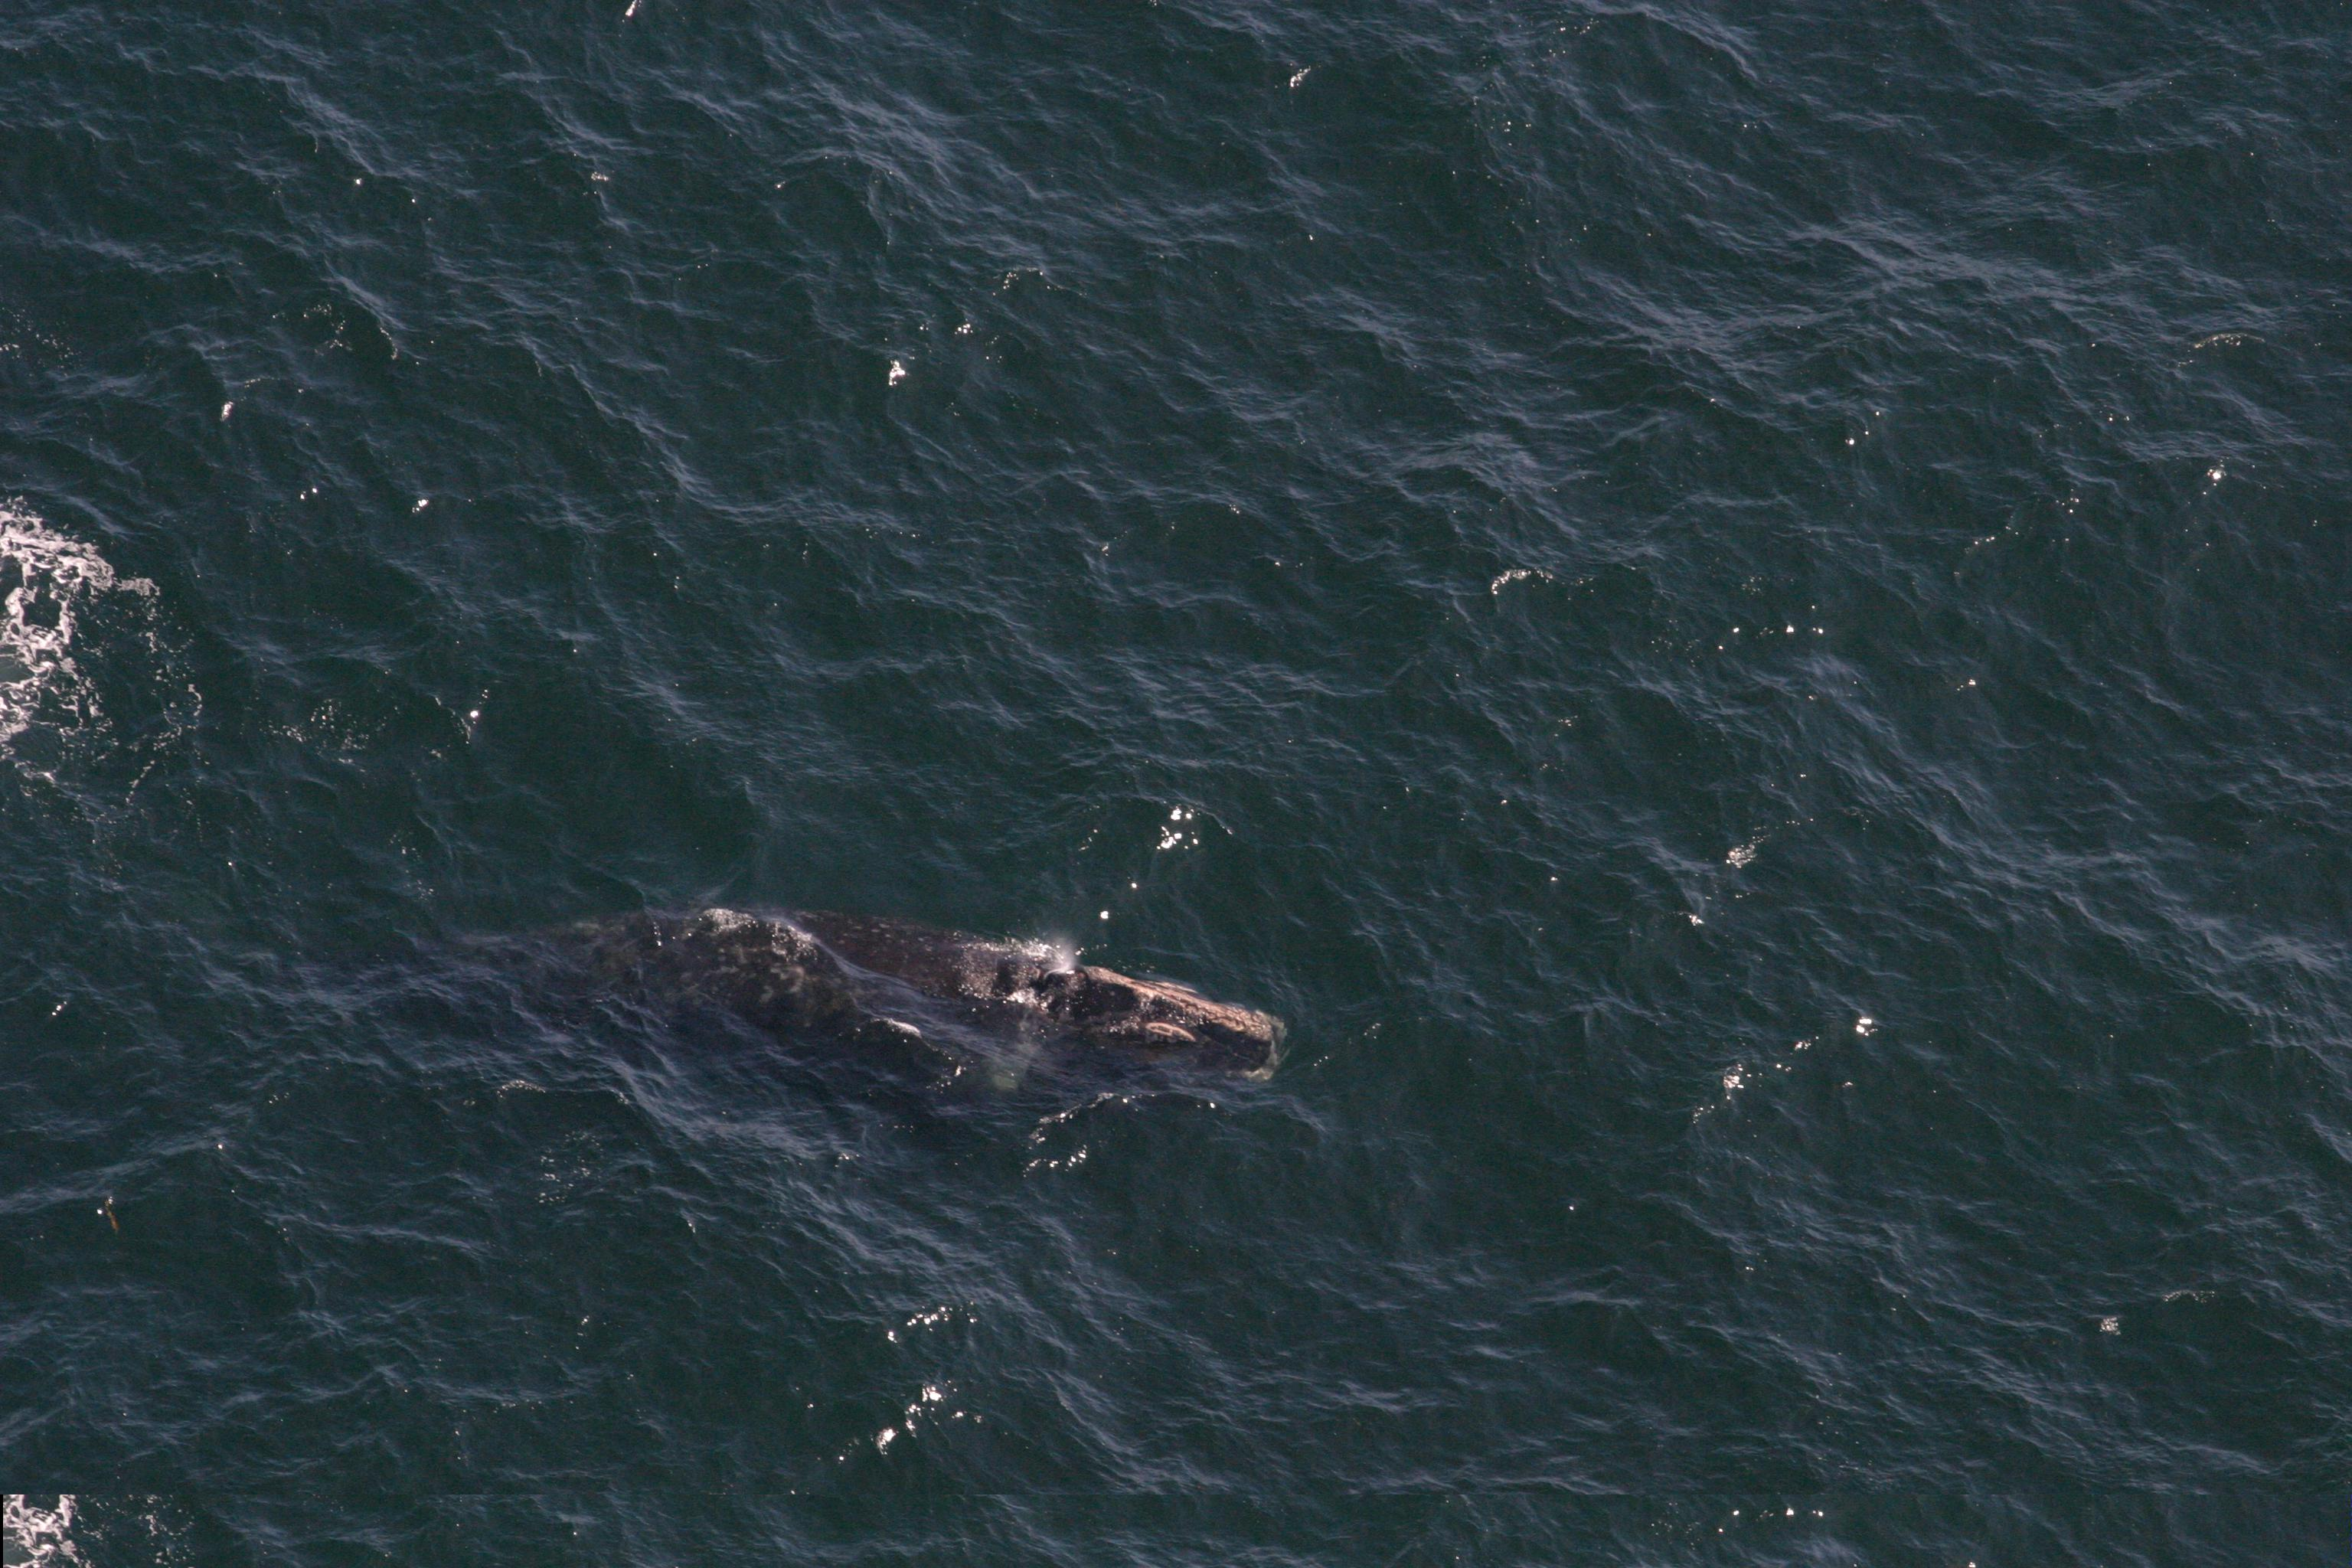
\includegraphics[width=\linewidth]{Images/w_7489}
	\caption{Example of whale from the dataset}
	\label{fig:whale-example}
\end{figure}

Another important thing to note about the dataset is the distribution of unique whales within the training data, an illustration of this can be seen in Figure \ref{fig:whale-frequency}. From this distribution it is notable that some whales are present in more images compared to some of the other whales. The results of the distribution can be seen in Table \ref{table:whale-distribution} where the minimum number of occurrences for a whale is 1 and the maximum is 47 with an average of 10,47 and a standard deviation of 6,8.

\begin{table}
	\centering
	\caption{Unique distribution of whales in the dataset}
	\label{table:whale-distribution}
	\begin{tabularx}{\linewidth}{|X|X|}
		\hline
		Min    & 1     \\ \hline
		Q1     & 5     \\ \hline
		Median & 9     \\ \hline
		Mean   & 10,17 \\ \hline
		Q3     & 14    \\ \hline
		Max    & 47    \\ \hline
		SD     & 6,8   \\ \hline
	\end{tabularx}
\end{table}

\begin{figure}
	\centering
	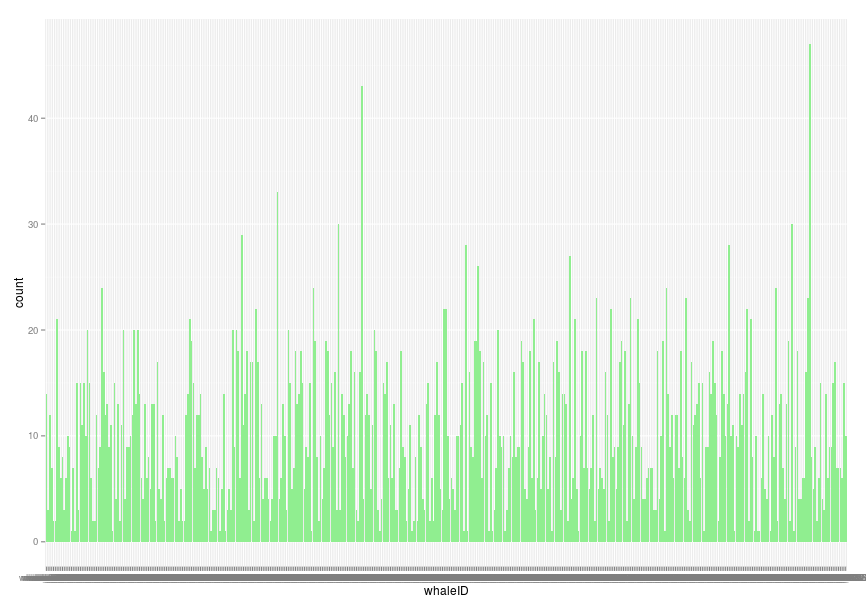
\includegraphics[width=\linewidth]{Images/FrequencyPlot}
	\caption{Frequency of unique whales in the training data}
	\label{fig:whale-frequency}
\end{figure}	